The testing implementation was developed with high modularity in mind,
since it is meant to be a proof-of-concept implementation and not a
production grade system. High modularity also makes development easier
and the system more robust against changes, two very important
qualities during this project.

The implementation is written in Python using NumPy and SQLite3, and
consists of three main parts:
\begin{description}
  \item[Particle Filter] A direct  implementation of the procedure in
    table \ref{alg:pf}.
  \item[Database] A database with functions for extracting transition
    hypotheses. Provides the prediction PDF $\cprobnext{x}$ to the
    particle filter.
  \item[Tracker] Manages the model and performs matching between
    hypotheses and images. Provides the filtering PDF
    $\cprob{I_n}{x_n}$ to the particle filter.
\end{description}

\section{The particle filter}
The particle filter implementation is a direct implementation of the
procedure in table \ref{alg:pf}. It is implemented as a function that
takes the parameters $X_{t-1}$, $I_t$, \texttt{importance\_function} and
\texttt{sampling\_function}. The parameters are the hypotheses from
the last time step, the current video frame and the functions to use
as \textsc{Predict} and \textsc{Importance} in \ref{alg:pf},
respectively. This means that the particle filter function is general
and independent of the model used. The implementations of
\textsc{Predict} and \textsc{Importance} are provided by the database
and tracker, respectively.

\subsection{Initilization $x_0$}
The test implementation needs to be manually initialized. When
tracking generated whiskers, the states were always known and the
initialization could therefore be programmatically inserted. When
testing on real whiskers, the start states were calculated by manually
selecting five or six pixels along each whisker and using a MATLAB
script to find the least squares solution for the coefficients
$\coeffs$. The problem of automatic
initialization is a difficult one \cite{Hedvig}, and is not covered in
this thesis.

\section{The state transition database}

\subsection{Data format}
A \emph{state transition} is a pair $\trans$ that denotes we have
observed a system go from state $\tf$ to state $\tt$ in one time
step. Technically, the state transition database is implemented as an
SQLite3 database. One transition is represented in the database as a
row with the state parameters of the model before and after the
transition. The set of transitions in the database will be denoted \TS.

\subsection{Prediction $\cprobnext{x}$}

\begin{table}[h]
  \begin{codebox}
    \Procname{$\proc{DB-Predict} (x_{t-1})$}
    \li $ x_t \gets 0$
    \li $ W \gets 0$
    \li \ForEach $(\tf, \tt) \in \TS$
    \li \Do
      \li $ w \gets \left(\Lpnorm[p]{\tf - x_t}\right)^{-a}$
      \li $ x_t \gets x_t + w \cdot \tt$
      \li $ W \gets W + w$
    \End
    \li Take $v \sim \ndist{0}{\Sigma}$
    \li \Return $ x_t / W + v $
  \end{codebox}
  \caption{Pseudocode for the prediction function. Notice the parameters $a$ and $p$.}
  \label{alg:predict}
\end{table}

The \textsc{Predict} function in table \ref{alg:pf} is implemented as
a weighted mean of the state transitions in the database. The function
is stated in table \ref{alg:predict}. Notice the parameters $a$ and
$p$. $p$ is a positive integer that determines which $\Lp$ space to
compute the norm in. $a$ is a positive number, and determines how fast
the weight $w$ declines with the distance $\Lpnorm[p]{\tf -
  x_{t-1}}$. A high $a$ means closer transitions get a much higher
weight than ones far away, see figure \ref{fig:x-to-the-minus-a}.

At this point, however, the prediction is still deterministic - the
result for any given input $x_{t-1}$ is completely determined by the
parameters $a$ and $p$ and the content of the database. A
deterministic prediction function is not desirable, since the
filtering step only removes improbable hypotheses and replaces them
with duplicates of probable ones. This means that having a
deterministic prediction effectively reduces the number of hypotheses
with each filtering step. For this reason, the result is offset by a
small normal distributed term\footnote{The offset $v$ is a polynomial
  $\Spline[b]{\omega}$ where coefficient $b_i \sim \ndist{0}{\sigma_i}
  $ and $\sigma_i$ is different for the different $i$.} $v$ to make
the prediction nondeterministic.

\begin{figure}[ht]
  \centering
  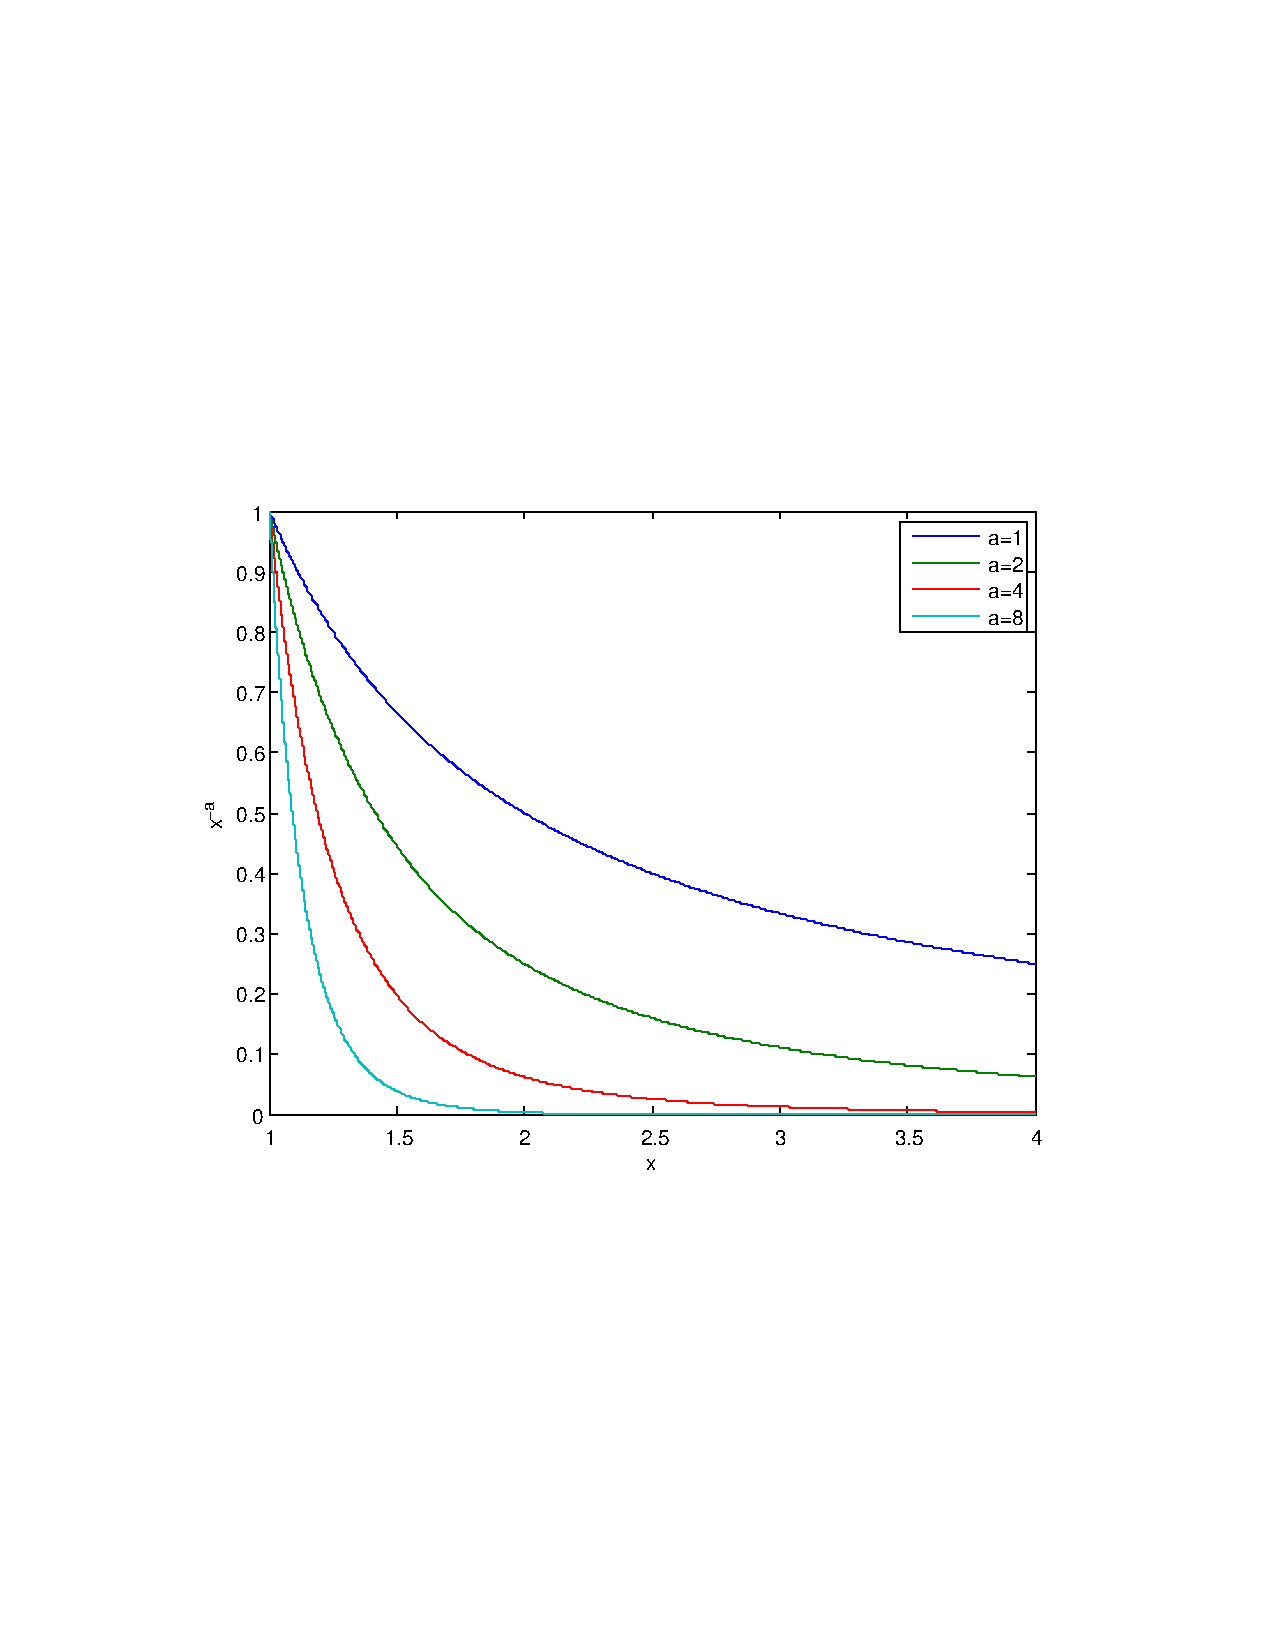
\includegraphics[width=0.4\textwidth,trim=65mm 65mm 65mm 65mm]{x-to-the-minus-a.pdf}
  \caption{Transitions closer to $x_{t-1}$ recieve a much greater
    weight if $a$ is large.}
  \label{fig:x-to-the-minus-a}
\end{figure}

\section{Tracker}

The tracker uses the whisker model described in chapter 4 and
internally represents whiskers with the tuple $\coeffs$ of polynomial
coefficients.

\subsection{Filtering $\cprob{I_t}{x_t}$}
\label{sec:filtering}
The \textsc{Importance} function in table \ref{alg:pf} is implemented
simply as the response of $x_t$ on $I_t$, raised to a power $g$. A
high $g$ means that the peak in the response is further
amplified. Figure \ref{fig:example-mask} shows an example of a
rendered hypothesis, as used for computing the response. See section
\ref{sec:response} for details on the response.

\begin{table}[h]
  \begin{codebox}
    \Procname{$\proc{Importance} (x_t, I_t)$}
    \li \Return $\Response{x_t}{I_t}{\phi}^g$
  \end{codebox}
  \caption{Pseudocode for the importance function. Notice the parameter $g$.}
  \label{alg:importance}
\end{table}

The \textsc{Importance} function in table \ref{alg:pf} as being the response for $x_t$ on $I_t$.
\begin{figure}[h]
  \centering
  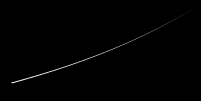
\includegraphics[width=0.38\textwidth]{example-mask.png}
  \caption{Example rendered image $R(x_t)$ for some hypothesis $x_t$.}
  \label{fig:example-mask}
\end{figure}

To indicate how the response works for generated and realdata we look at the following figures.
Figure \ref{fig:response_generated} shows the response curve for a generated image with parameters $(0,0,0)$ when varying the different parameters in the polynomial model.
Figure \ref{fig:response_real} shows the response curve for real images which has approximatly the parameters $(0,0,0)$, we can clearly see that the curve is far from perfect. 
The ground truth peak is still around $(0,0,0)$ but much less appearent.
The faulty peeks is generated by clutter from the other whiskers and we can see a tendency for higher values for positive $a_2,a_3$ which is probably due to motion blur effects.

\begin{figure}
    \centering
    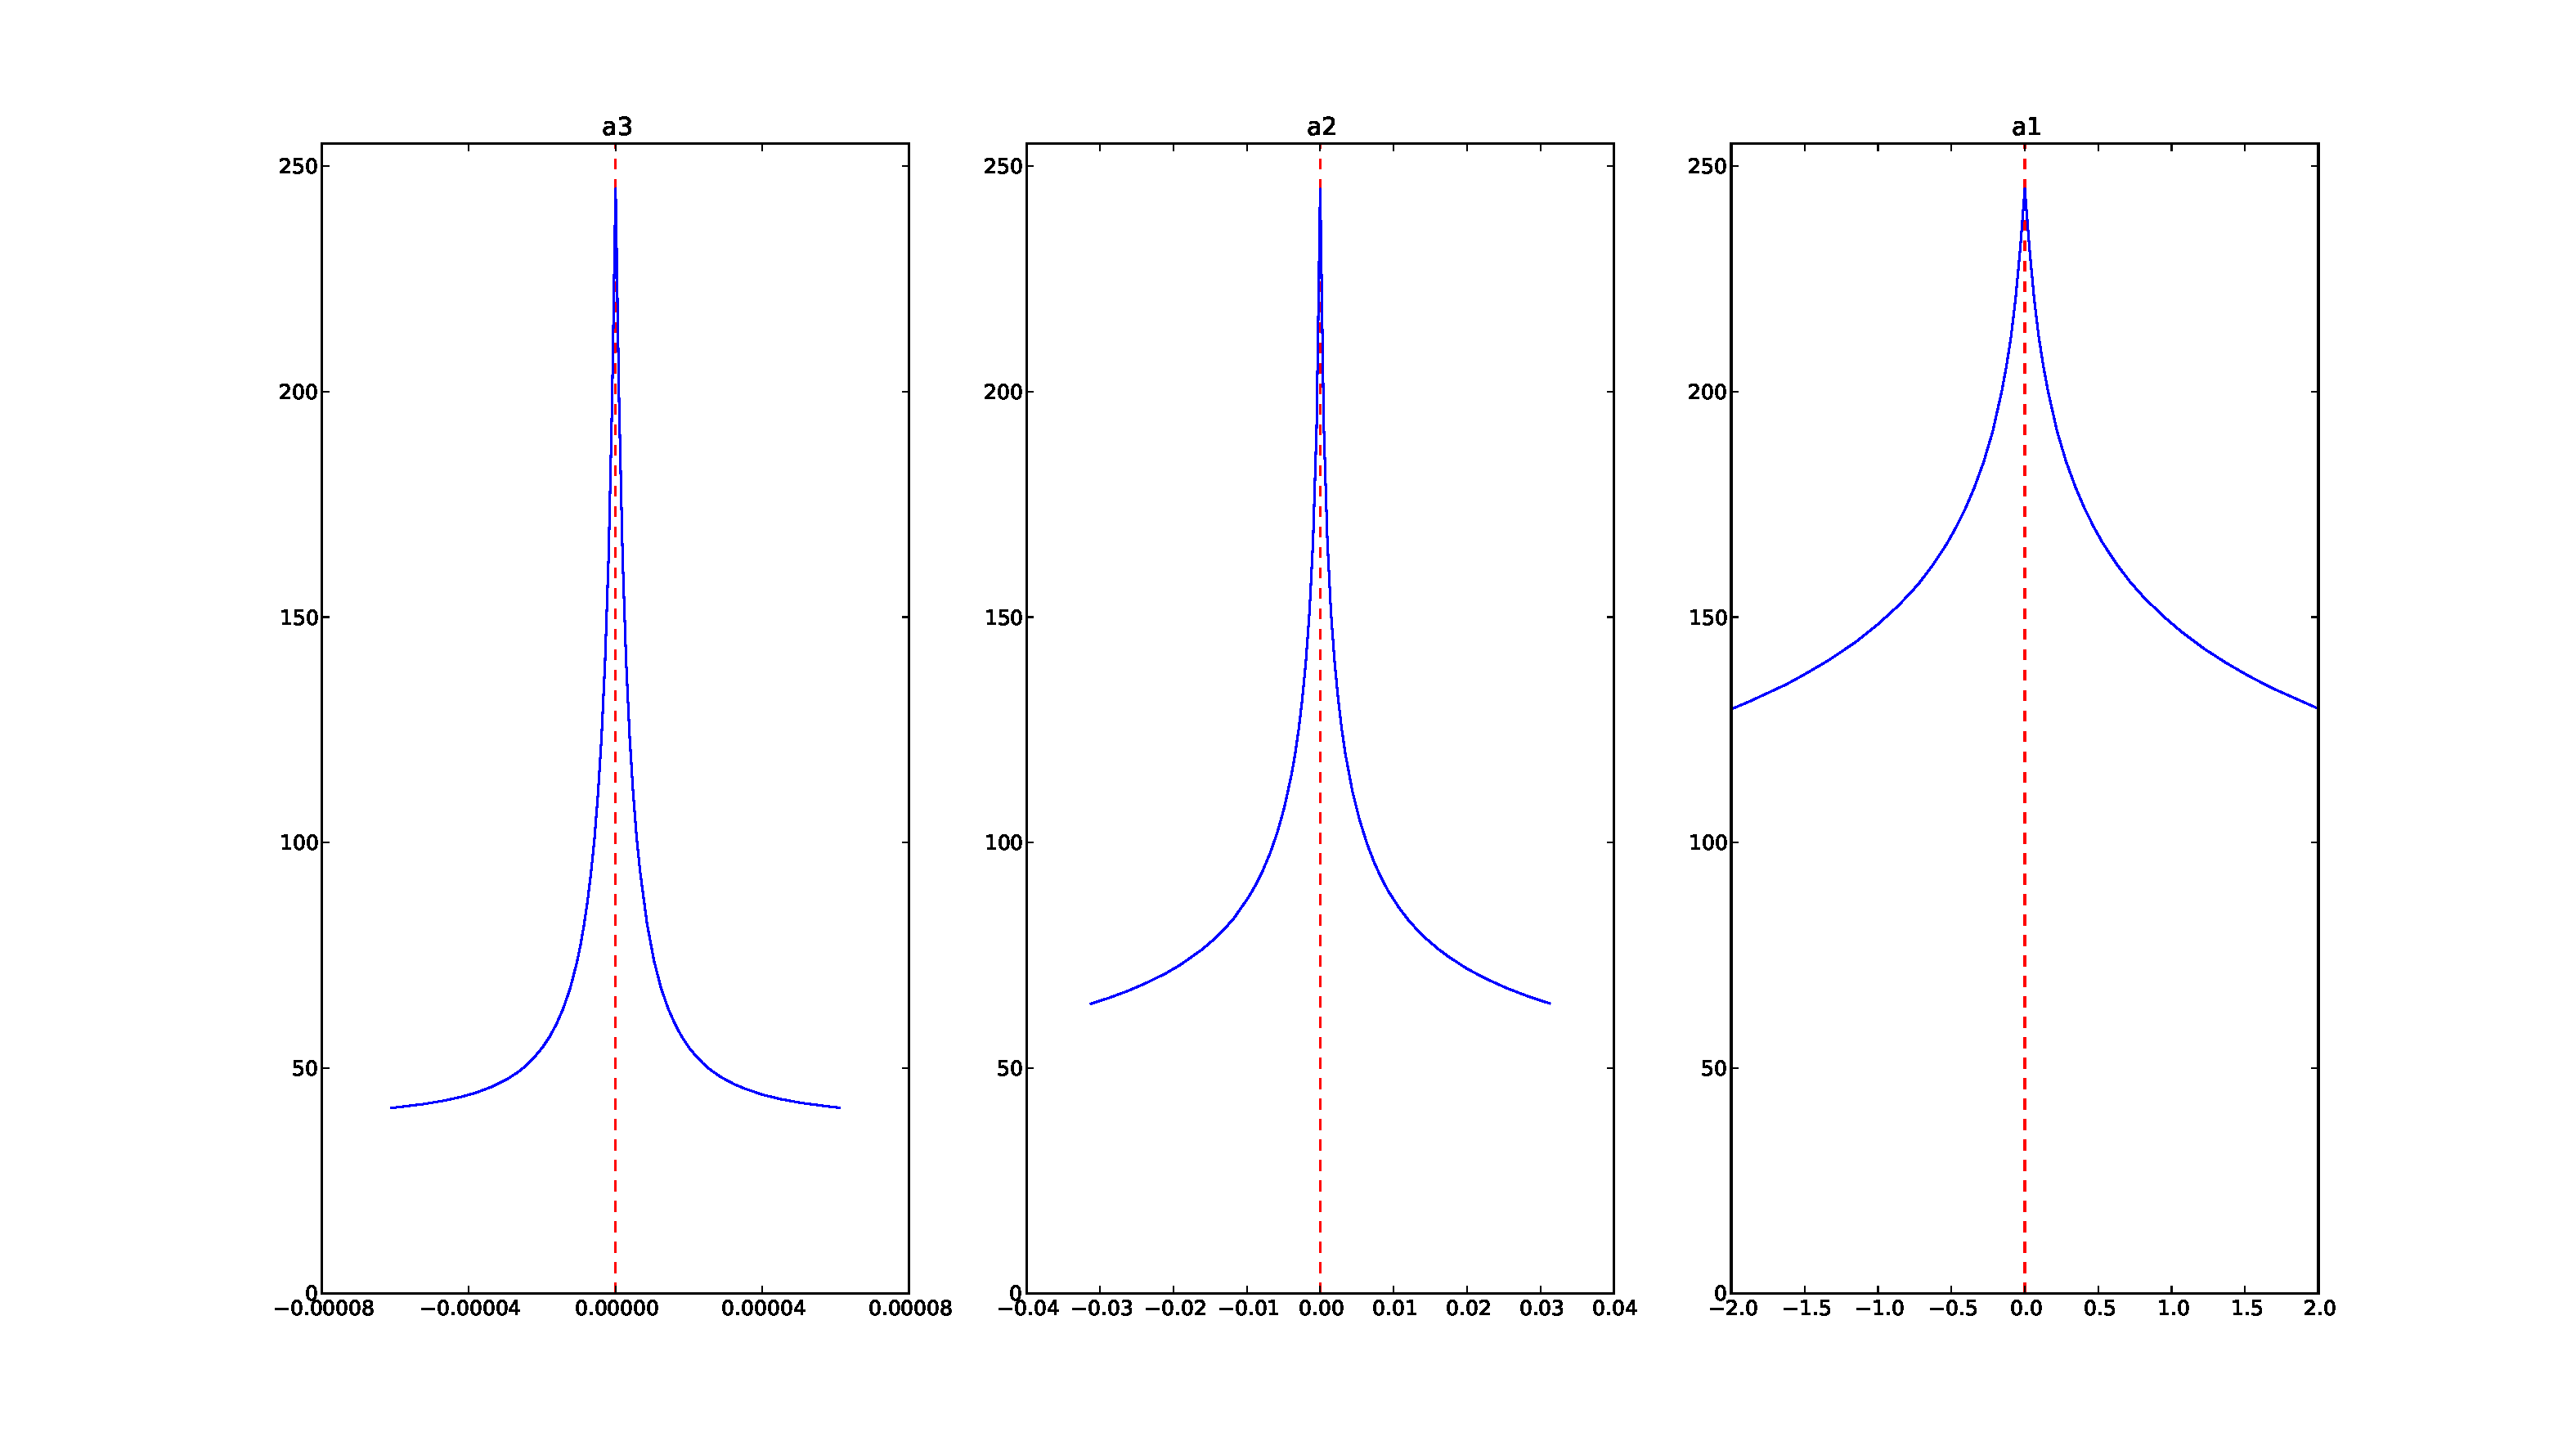
\includegraphics[width=\textwidth]{response_curves.pdf}
    \caption{
        Response curves over the parameters $(a_3,a_2,a_1)$ of the polynomial model on a generated whiskers image with the parameters $(0,0,0)$. With $\phi=1$.
    }
    \label{fig:response_generated}
\end{figure}
\begin{figure}
    \centering
    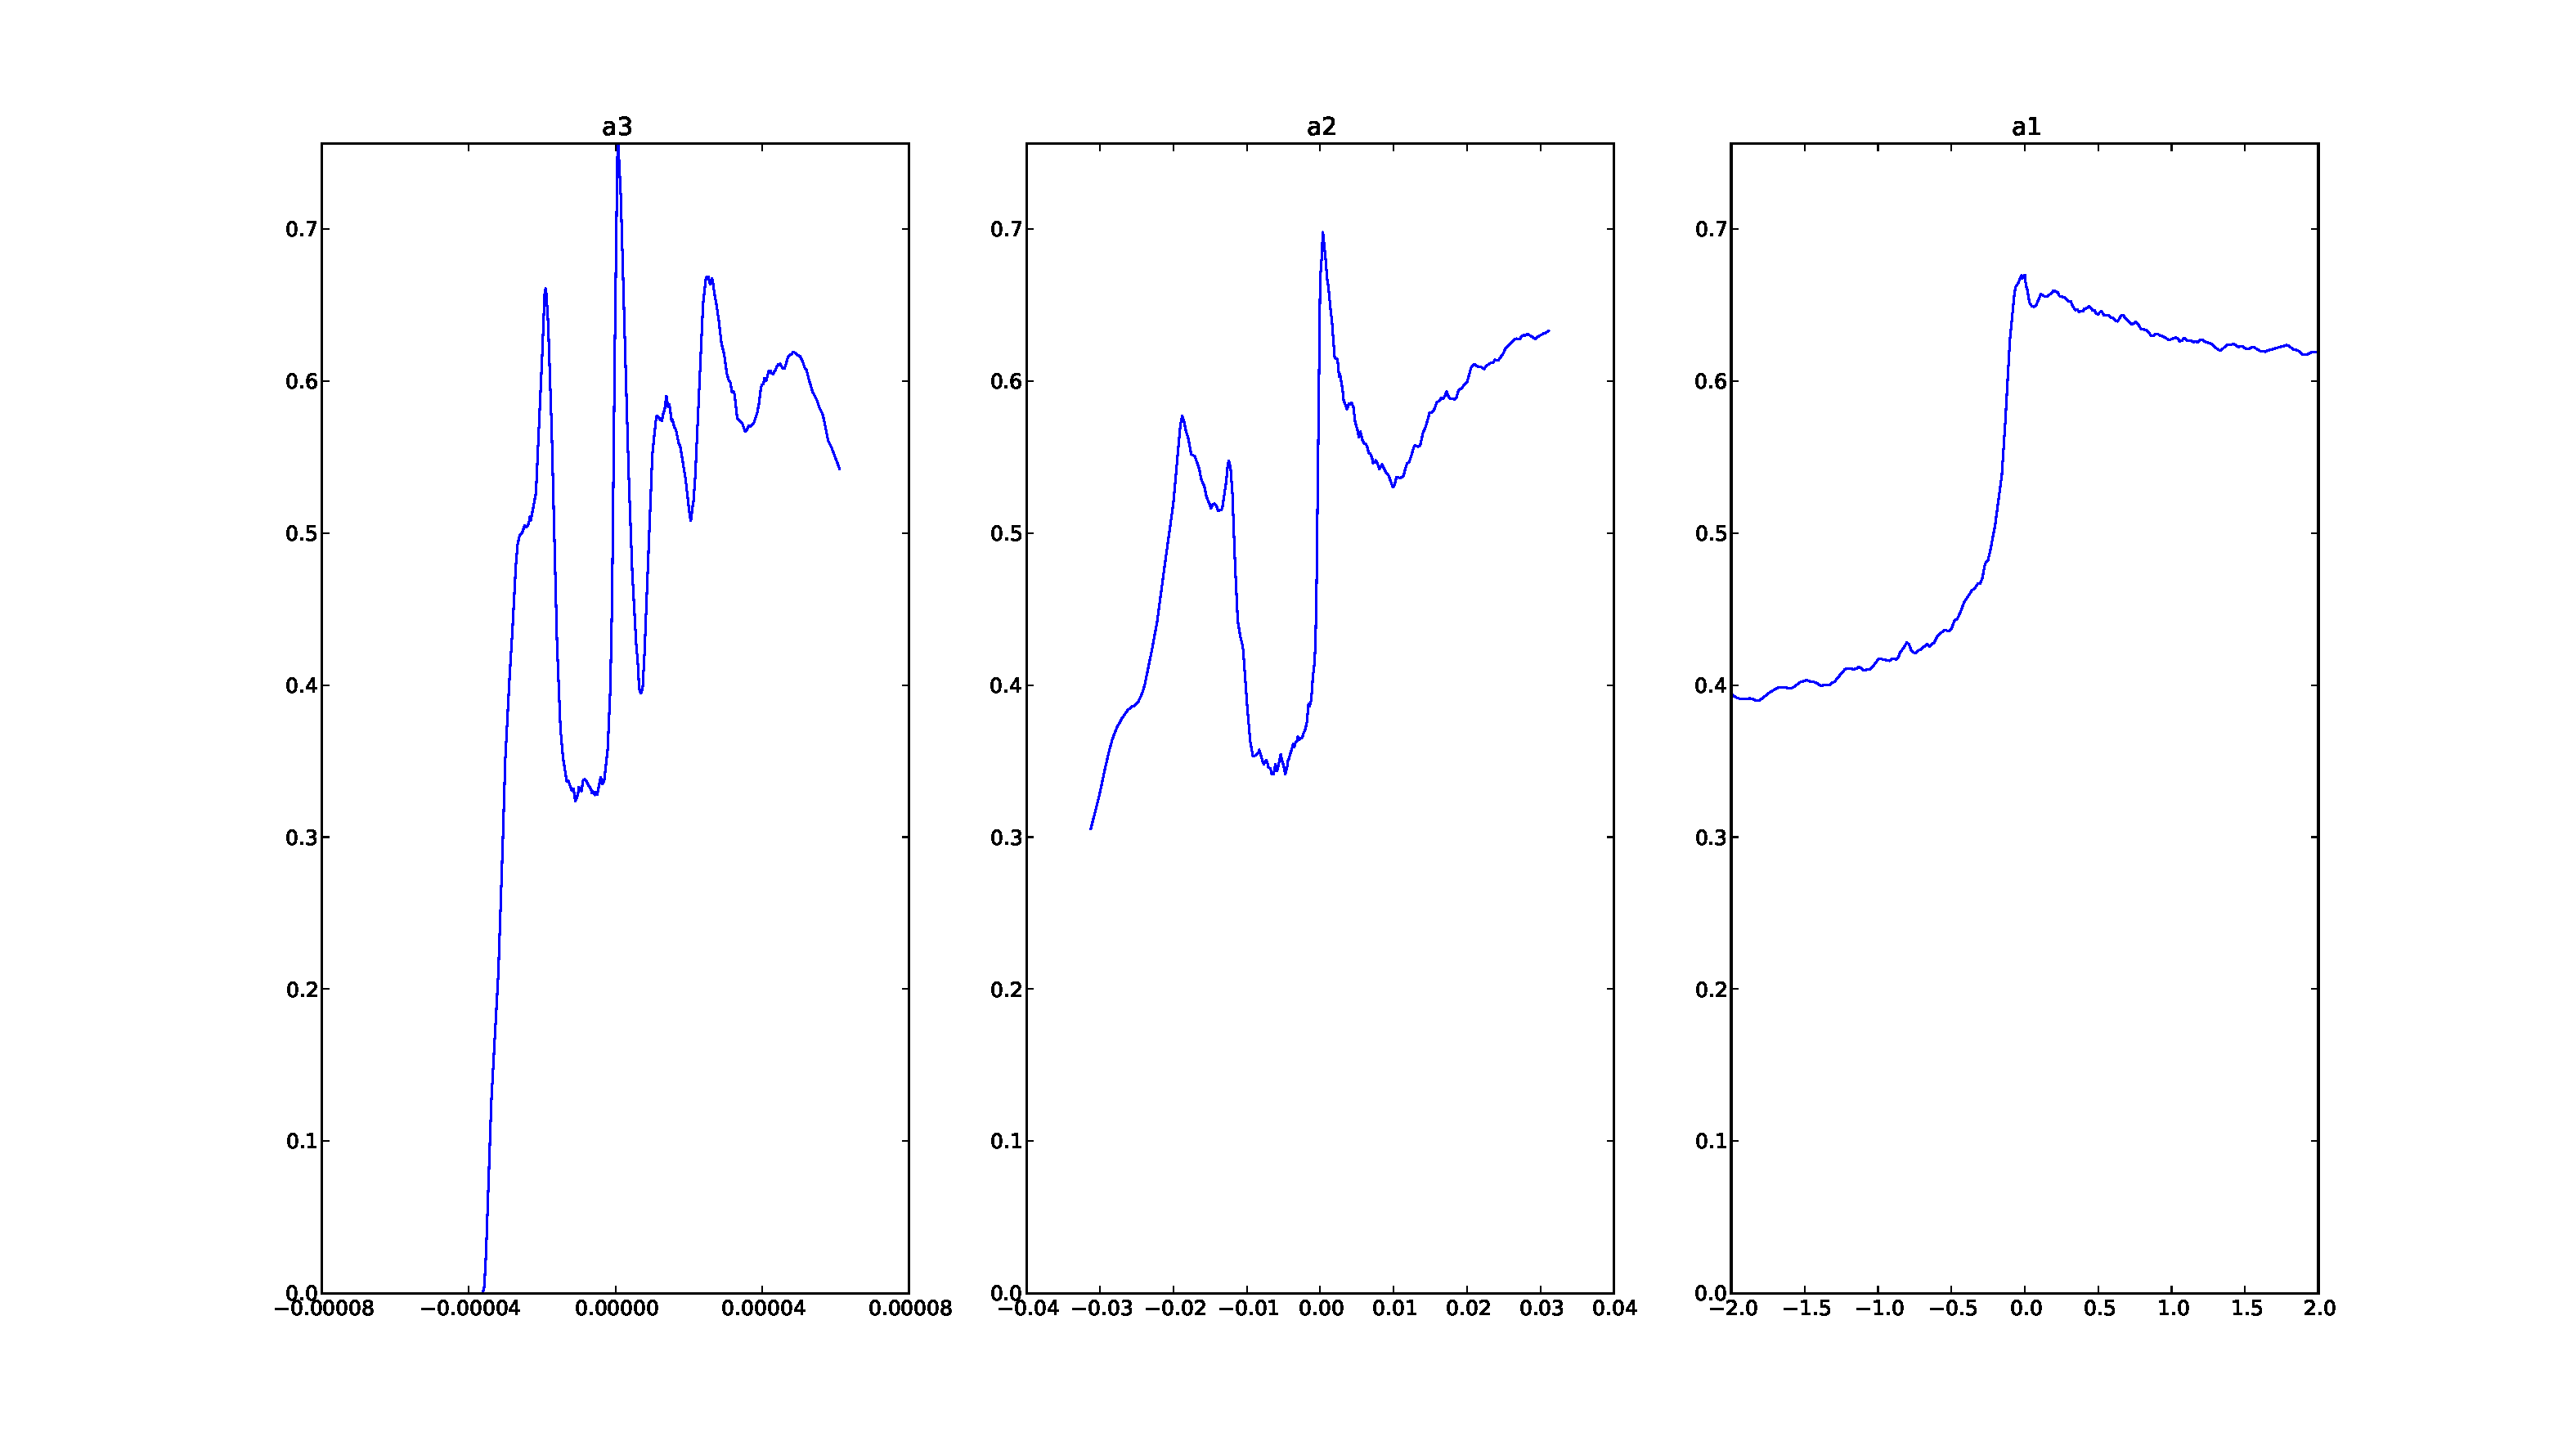
\includegraphics[width=\textwidth]{response_curves_real.pdf}
    \caption{
        Response curves over the parameters $(a_3,a_2,a_1)$ of the polynomial model on a real whisker image, $\prob{whisker}$ from \ref{sec:findwhisker},
        with approximatly the parameters $(0,0,0)$. With $\phi=1$.
    }
    \label{fig:response_real}
\end{figure}

\section{Preprocessing of real images}
\label{prep-real}

In the images of real rodents used for testing, the rodent was
illuminated from below, meaning it and its whiskers were dark against
a bright background as in the figure \ref{fig:original_bg}. The filtering function described in the previous
section expects whisker pixels to be bright, so the images had to be
inverted. However, the body had the same pixel values as the whiskers,
meaning no conclusions can be drawn simply by inspecting the value of
a pixel. Therefore the following steps also had to be taken.

\subsection{Background subtraction}
Removing effects like difference in background illumination and static
objects is preferred in order to minimize faulty responses.

Assuming we always have a static camera setup for each sequence and
that we have an adequate sequence without the rodent, the background
$BG$ was captured a priori by taking the mean $I_{BG}$ of the first
100 frames as seen to the left in figure \ref{fig:orignal_bg}.\footnote{A sufficient number} Then we can simply subtract
the background $I_{BG}$ from the orignal image $I$ and getting the result shown to the right in figure \ref{fig:subtract}: \footnote{Worth
noting is that more sophisticated background subtraction methods
exist, but this solution works relatively well considering the
simplicity.}

\begin{equation}
  I_{FG} = I - I_{BG}.
\end{equation}

\begin{figure}
\begin{center}
    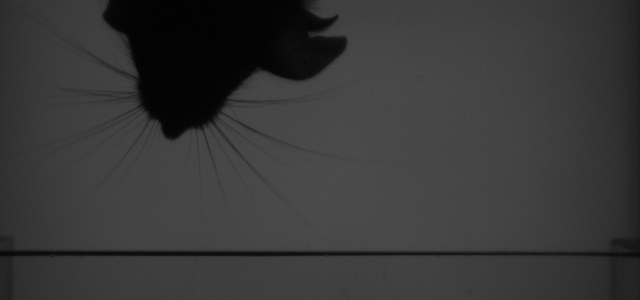
\includegraphics[width=0.45\textwidth]{frame-0759.png}
    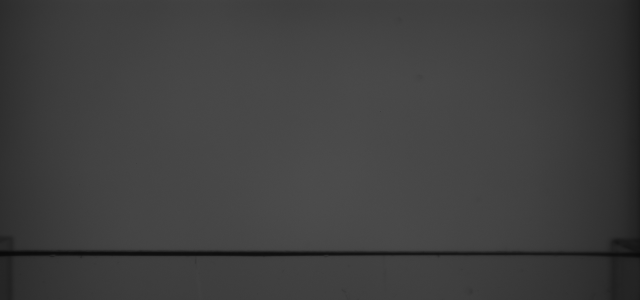
\includegraphics[width=0.45\textwidth]{frame-0759_bg.png}
\end{center}
\caption{The image to the left shows the original image, to the right we have the mean static background.}
\label{fig:orignal_bg}
\end{figure}
\begin{figure}
\begin{center}
    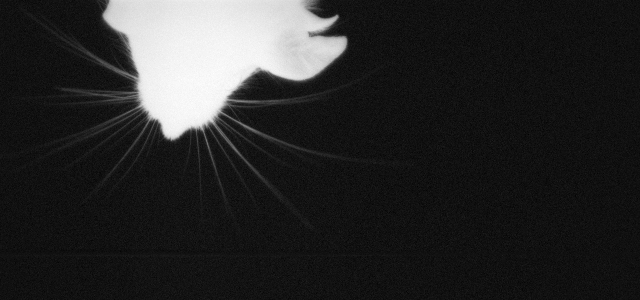
\includegraphics[width=\textwidth]{frame-0759_sub.png}
\end{center}
\caption{The image shows the effect of subtracting the static background.}
\label{fig:subtract}
\end{figure}

\subsection{Extract the body $\prob{\text{body}}$}
\label{sec:findbody}
Extracting the body has two purposes. First, to find the head-fixed
coordinate system. Second, to subtract the body from the image in
order to highlight the whiskers.

\begin{definition}
  The image
  \begin{equation}
    \prob{\text{body}}\in \IS
  \end{equation} is an estimation if the probablity of the pixel
  being a body pixel.\footnote{The estimate only needs to
    be an indication of whether it is a body}
\end{definition}

We will assume that the only non-static objects in the image are the
whiskers and body. One simple feature that easily classifies
$\prob{\text{whisker}}$ from $\prob{\text{body}}$ is size. Blurring
the image removes fine structures and retains larger which can be seen to the left in figure \ref{fig:blured_snout}.  This was
performed by convoluting the image with a Gaussian with
${\sigma=9}$px:\footnote{The value of $\sigma$ was obtained by manual
  testing and inspection.}

\begin{equation}
  \prob{\text{body}} = I_{blur} = I_{FG} \star \ndist{0}{\sigma}.
\end{equation}
Note that $\ndist{\mu}{\sigma}$ traditionally denotes a set of normal
distributed stochastic variables. In this thesis, we will also use
this to denote the PDF of the normal distribution, and let the context
provide the distinction.

$\prob{\text{body}}$ was then used to create a \emph{mask} $I_{\text{body}}$:
\begin{equation}
  I_{\text{body}} = \prob{\text{body}}>0.6 \in \IS,
\end{equation}
meaning $I_{\text{body}}$ is white where $\prob{\text{body}}$ is greater than
0.6 and black everywhere else, the result is displayed to the right in figure \ref{fig:blured_snout}.\footnote{The 0.6 threshold was found,
through manual testing, to make the body stable between frames.}

\begin{figure}
\begin{center}
    
\includegraphics[width=0.45\textwidth]{frame-0759_blured.png}
    
\includegraphics[width=0.45\textwidth]{frame-0759_snout.png}
\end{center}
\caption{The image to the left shows the blured image with ${\sigma=9}$px, to the right we have the snout mask.}
\label{fig:blured_snout}
\end{figure}

\subsection{Extract the whiskers $\prob{\text{whisker}}$}
\label{sec:findwhisker}
The filtering described in section \ref{sec:filtering} needs an
indicator for the locations of whiskers.

\begin{definition}
  The image
  \begin{equation}
    \prob{\text{whisker}}\in \IS
  \end{equation} is an estimation of the probablity of a pixel being
  a whisker pixel.\footnote{The estimate only needs to be an
    indication of whether it is a whisker.}
\end{definition}

This is naively performed by masking with the inverse
$\bar{I}_{\text{body}}$ of $I_{\text{body}}$:

\begin{equation}
  \prob{\text{whisker}} = I_{FG} * \bar{I}_{\text{body}}
\end{equation}
which finally gives the results shown in figure \ref{fig:whiskers}.

\begin{figure}
\begin{center}
    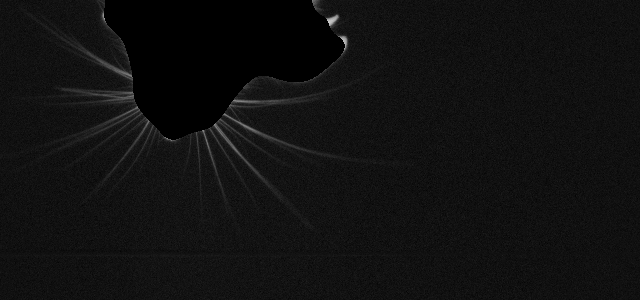
\includegraphics[width=\textwidth]{frame-0759_whiskers.png}
\end{center}
\caption{The finished preprocessed image.}
\label{fig:whiskers}
\end{figure}

\subsection{Find the snout coordinate system}
The whisker model does not take head movements into account, and
therefore expects whisker roots to be stationary throughout the
sequence. Therefore, the video is translated such that the head stays
approximately fixed throughout the image sequence.

For this, we use a transformation $\phi$ that extracts the shape of
the body. $\phi$ first blurs the image\footnote{The value $\sigma = $
  5 pixels was obtained through manual testing.}, to smooth out the
response, then applies a Prewitt filter:
\begin{IEEEeqnarray*}{rCl}
  \phi_{\text{blur}}(I) &=& I \star \ndist{0}{5\mathrm{px}}\\
  \phi(I) &=& \sqrt{(\phi_{\text{blur}}(I) \star \text{Prewitt}_x)^2 +
    ( \phi_{\text{blur}}(I) \star \text{Prewitt}_y )^2}.
\end{IEEEeqnarray*}
that extracts the shape of the body.

The first frame where the snout is fully visible is hand picked
and used to create an image $I_{\text{ref}} = \phi(I_{\text{body}})$,
where $I_{\text{body}}$ is created through the steps detailed in
section \ref{sec:findbody}.

A local search within $5$px from the last location is then
performed\footnote{This could easily be extended to include rotation
  as well.} for each body image $I_{\text{body}}$ in the
sequence, which can be seen in figure \ref{fig:tracked_snout}. The translation $(\Delta x, \Delta y)$ from $I_{\text{ref}}$
is extracted:\footnote{In the same way as $\Response{\cdot}{\cdot}{\phi}$ but without the hypothesis.}
\begin{equation}
  (\Delta x, \Delta y) = \argmax{(x,y)~\text{close}}
  (\sum 
  \text{translate}(I_{\text{ref}},-(x,y))*\phi(I_{\text{body}})
  )
  \in \ZZ^2,
\end{equation}
and the frame is then translated accordingly.

\begin{figure}
\begin{center}
    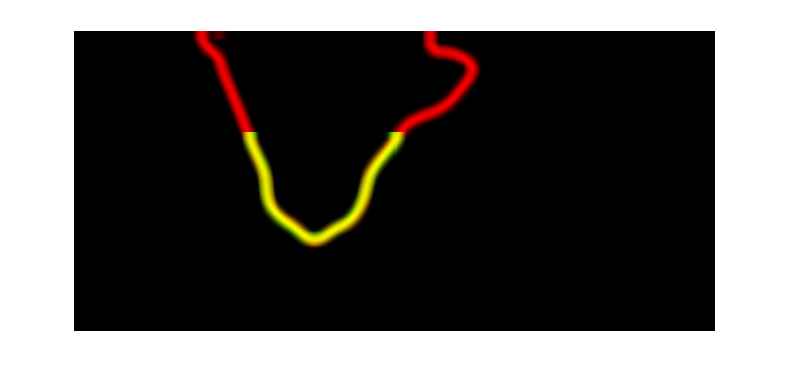
\includegraphics[width=\textwidth]{snout_tracked.png}
\end{center}
\caption{Showing the snout coordinate system tracking in progress, the best match is shown. Reference image is in green and the tracked image is red, the overlapping becomes yellow.}
\label{fig:tracked_snout}
\end{figure}


